\documentclass[10pt]{article}

%TITLE
%=====
\title{\huge{\textbf{Two Dimensional \\ \vspace{1cm} protodns code}}}
\author{}
\date{}
%PAGE LAYOUT
%===========
\setlength{\oddsidemargin}{0pt}
\setlength{\evensidemargin}{0pt}
\setlength{\marginparwidth}{0pt}
\setlength{\marginparpush}{0pt}
\setlength{\marginparsep}{0pt}
\setlength{\textwidth}{464pt}
\addtolength{\topmargin}{-2.0cm}
\addtolength{\textheight}{4.0cm}

%PACKAGES
%========
\usepackage{bm}
\usepackage{amsmath}
\usepackage{mathrsfs}
\usepackage{amsfonts}
\usepackage{graphicx}
\usepackage{booktabs}
\usepackage{hyperref}
\usepackage{colordvi,color}

%MACRO DEFINITION
%================
\def\dotp{\bm{\cdot}}
\def\crossp{\bm{\times}}
\def\grad{\bm{\nabla}}
\def\div{\bm{\nabla\cdot}}
\def\curl{\bm{\nabla\times}}
\def\lap{{\nabla}^2}
\def\lapinv{{\nabla}^{-2}}
\def\so{\quad\Rightarrow\quad}
\def\soo{\qquad\Rightarrow\qquad}
\def\A{\bm{A}}
\def\S{\bm{S}}
\def\F{\bm{F}}
\def\p{\bm{p}}
\def\q{\bm{q}}
\def\r{\bm{r}}
\def\u{\bm{u}}
\def\x{\bm{x}}
\def\OMEGA{\bm{\omega}}
\def\eI{\bm{\hat{i}}}
\def\eJ{\bm{\hat{j}}}
\def\eK{\bm{\hat{k}}}
\def\en{\bm{\hat{n}}}

%COMMANDS OPTIONS
%================
\definecolor{heavyred}{cmyk}{0,1,1,0.25}
\definecolor{heavyblue}{cmyk}{1,1,0,0.25}
\hypersetup{
  pdftitle=Clebsch Vector Potential,
  pdfpagemode=UseOutlines,
  citebordercolor=0 0 1,
  colorlinks=true,
  allcolors=heavyred,
  breaklinks=true,
  pdfauthor={Pedram Emami},
  pdfpagetransition=Dissolve,
  bookmarks=true
}

%BODY OF THE DOCUMENT
%====================
\begin{document}
\maketitle
The main advantage of solving vorticity equation instead of momentum equation is the fact that vorticity equation does not involve pressure term which in turn involves solving Poisson's equation, so for our purpose which is direct numerical simulation of isotropic homogeneous turbulence, taking this approach makes it possible to have faster numerical simulation. Considering vorticity equation, we would have :
%
%====================== Eq-1
\begin{equation}\label{Eq-1-Vorticity}	
\frac{\partial{\OMEGA}}{\partial t} + (\u\dotp\grad)\OMEGA=(\OMEGA\dotp\grad)\u + \nu\lap\OMEGA + \curl\F
\end{equation}
%
now for the case of 2D incompressible fluid flow we have:
%
%====================== Eq-2
\begin{equation}\label{Eq-2}
\u=u(x,y)\eI+v(x,y)\eJ, \qquad \div\u=0
\end{equation}
%
so it is well known that for this type of fluid flow we can represent the velocity field by using stream function $\psi$ such that:
%
%====================== Eq-3
\begin{equation}\label{Eq-3}
u=-\frac{\partial\psi}{\partial y},\quad v=\frac{\partial\psi}{\partial x}
\end{equation}
%
now by the definition of vorticity which is $\OMEGA=\grad\crossp\u$, then we will have:
%
%====================== Eq-4
\begin{equation}\label{Eq-4}
\OMEGA=\left(\frac{\partial v}{\partial x}-\frac{\partial u}{\partial y}\right)\eK
\end{equation}
%
which in fact shows that in the case of 2D incompressible fluid flow, $\OMEGA$ is a vector whose direction is always prependicular to the velocity vector, so what is matter regarding the velocity vector is its length. Thus, we can look at the vorticity as an scalar. Now using the equation \eqref{Eq-3} in \eqref{Eq-4}, we will have:
%
%====================== Eq-5
\begin{equation}\label{Eq-5}
\OMEGA=(\lap\psi)\eK
\end{equation}
%
while we can write:
%
%====================== Eq-6
\begin{equation}\label{Eq-6}
\u=\frac{\partial\psi}{\partial y}\eI+\frac{\partial\psi}{\partial x}\eJ=\eK\crossp\grad\psi
\end{equation}
so using equations \eqref{Eq-5},\eqref{Eq-6}, we can represent the velocity vector with respect to the stream function and consequently the vorticity as:
%
%====================== Eq-7
\begin{equation}\label{Eq-7}
\u=\eK\crossp\grad(\lapinv\omega)
\end{equation}
%
as we mentioned above, because in 2D fluid flow, the vorticity is always prependicular to the velocity, and also because of continuity, then the first term in the right hand side of the vorticity equation vanishes, so the vorticity equation becomes:
%
%====================== Eq-8
\begin{equation}\label{Eq-8}
\frac{\partial{\omega}}{\partial t} + (\u\dotp\grad)\omega= \nu\lap\omega + f
\end{equation}
%
now by expanding equation\eqref{Eq-8}, we would have:
%
%====================== Eq-9
\begin{equation}\label{Eq-9}
\frac{\partial{\omega}}{\partial t} + (\eK\crossp\grad(\lapinv\omega)\dotp\grad)\omega= \nu\lap\omega + f
\end{equation}
now using inverse discrete Fourier transform, we would have:
%
%====================== Eq-10
\begin{align}
\omega(\x)&=\sum_{\p}{e^{i\p\dotp\x}\omega(\p)}=\sum_{\p}{e^{i\p\dotp\x}\omega_{\p}} 		     \notag 
\\
(\eK\crossp\grad(\lapinv\omega(\x))\dotp\grad)\omega(\x) &=(\eK\crossp\grad(\lapinv\sum_{\p}{e^{i\p\dotp\x}\omega_{\p}})\dotp\grad)\sum_{\q}{e^{i\q\dotp\x}\omega_{\q}} 									 \notag 
\\
&=\sum_{\p,\q}{\frac{(\eK\crossp\p)\dotp\q}{|\p|^2}\omega_{\p}\omega_{\q}e^{i(\p+\q)\dotp\x}} \notag 
\\
\nu\lap\omega(\x)&=\nu\sum_{\p}{|\p|^2e^{i\p\dotp\x}\omega_{\p}} 								 \notag 
\\
f(\x)&=\sum_{\p}{e^{i\p\dotp\x}f_{\p}} \label{Eq-10}
\end{align}
%
now, using \eqref{Eq-10} and taking discrete Fourier transform of \eqref{Eq-9}, we have:
%
%====================== Eq-11
\begin{equation}\label{Eq-11}
\frac{\partial}{\partial t}({\sum_{\p,\r}{e^{i(\p-\r)\dotp\x}\omega_{\p}}}) + \sum_{\p,\q,\r}{\frac{(\eK\crossp\p)\dotp\q}{|\p|^2}\omega_{\p}\omega_{\q}e^{i(\p+\q-\r)\dotp\x}}= \nu\sum_{\p,\r}{|\p|^2e^{i(\p-\r)\dotp\x}\omega_{\p}} + \sum_{\p,\r}{e^{(i\p-\r)\dotp\x}f_{\p}}
\end{equation}
%
now by simplifying the above equation, the final governing equation in the wave space would be:
%
%====================== Eq-12
\begin{equation}\label{Eq-12}
\frac{\partial\omega_{\r}}{\partial t} + \sum_{\p}{\frac{(\eK\crossp\p)\dotp\r}{|\p|^2}\omega_{\p}\omega_{\r-\p}}= \nu{|\r|}^2\omega_{\r} + f_{\r}
\end{equation}
%
%====================== Fig-1
\begin{figure}
\centering
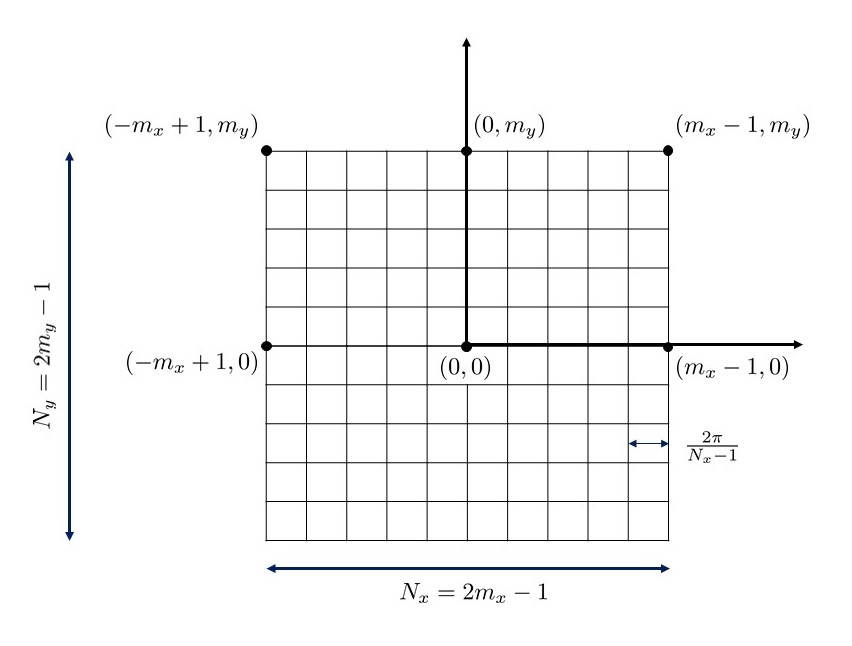
\includegraphics[scale=0.5]{domain}
\caption{Domain of simulation}\label{Fig-1}
\end{figure}
%
now as we want to study homogeneous isotropic turbulence, we have to avoid having walls or in fact we have to stay far enough from walls , so the best approach is to take our domain with periodic boundary conditions. In the schematic figure \ref{Fig-1}, our domain has been represented. Now using equation \eqref{Eq-12}, we can rewrite the equation as :
%
%====================== Eq-13
\begin{align}
\frac{\partial\omega_{\r}}{\partial t} &= -\sum_{\p}{\frac{(\eK\crossp\p)\dotp\r}{|\p|^2}\omega_{\p}\omega_{\r-\p}}+\nu{|\r|}^2\omega_{\r} + f_{\r} \tag*{} \\
&=: S_{\r}\label{Eq-13}
\end{align}
%
where $S_{\r}$ is the source term which is a function of $\omega_{\r}$. Now it is clear that the\eqref{Eq-13} is a first order ODE that can be solved using implicit time marching method. The main solution algorithm has been shown in \ref{Fig-2}. It should be noticed that \ref{Fig-2} is the most general solution algorithm while in action, many different optimization and generalizations must be added to the shown algorithm to make the final numerical simulation as most efficient(regarding CPU time and memory usage) as possible.
%
%====================== Fig-2
\begin{figure}
\centering
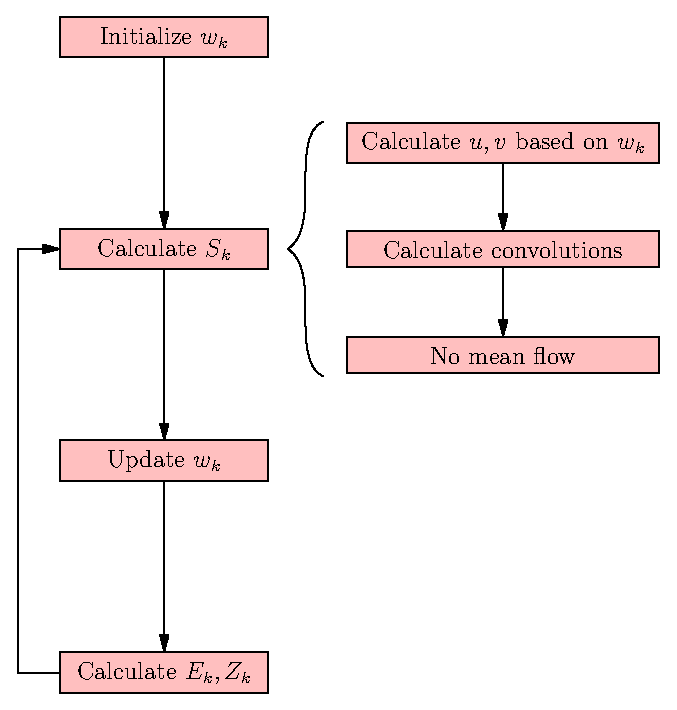
\includegraphics[scale=0.5]{algorithm}
\caption{Solution algorithm}\label{Fig-2}
\end{figure}
%
\end{document}





